%================================================================
\chapter{Inference on Hodgkin-Huxley}\label{chap:res_hh}
%================================================================  

In this chapter, we present the results from using simulation-based inference on the Hodgkin-Huxley (HH) model's conductance parameters $\gbarK$ and $\gbarNa$. 

%\url{https://github.com/mackelab/sbi/blob/main/examples/00_HH_simulator.ipynb}

%Chapter Inference on the HH model 

%- observed data (clean)
%- priors
%- prior predictive sum stats 
%- rej-abc analysis 
%- rej-abc (original) posteriors 
%- reg adj posteriors
%- ppc 

%- observed data noisy 
%- rej-abc (original) posteriors 
%- reg adj posteriors
%- ppc 

%- sbi

%reproducing AP
%numerical solutions similar
%capture

%================================================================
\section{Observation and Feature Extraction}
%================================================================

Let us assume we current-clamped a neuron and recorded the voltage trace in \autoref{fig:hh_obs_data}. This voltage trace was not actually measured experimentally but synthetically generated by simulating the HH model through the HH simulator in \cw{NeuroModels}. The model was simulated for $T=120\ms$ with step size $\Delta t =10 \ms$ and stimulus $I = 10 \, \mathrm{\mu A/cm}^2$ turned on at $10 \ms$ and off at $110 \ms$. The conductance parameters were set as $\gbarK=36 \gunit$ and $\gbarNa=120 \gunit$. The rest of the HH model's parametrization is given in \autoref{tab:hh_model_parameters}. The idealized voltage trace recording, free of any noise, will be used as the observed data in our first analyses. Hopefully, we can then more easily assess strengths and weaknesses of the algorithms themselves, and not have the results overshadowed by noisy data. Furthermore, the present trace allows us to verify whether the computational implementations are accurate. The ground truth parameters will therefore be the particular values of $\gbarK$ and $\gbarNa$ used in the simulation.  

By visual inspection of the trace in \autoref{fig:hh_obs_data}, the expected shape of an action potential (AP) is reproduced by the numerical solution, which indicates that the implementation of the simulator is accurate. Moreover, since the voltage trace does not display any unexpected abrupt behavior, the time resolution of $\Delta t=0.025 \ms$ seems to be sufficient. 

\begin{figure}[!htb]
    \centering
    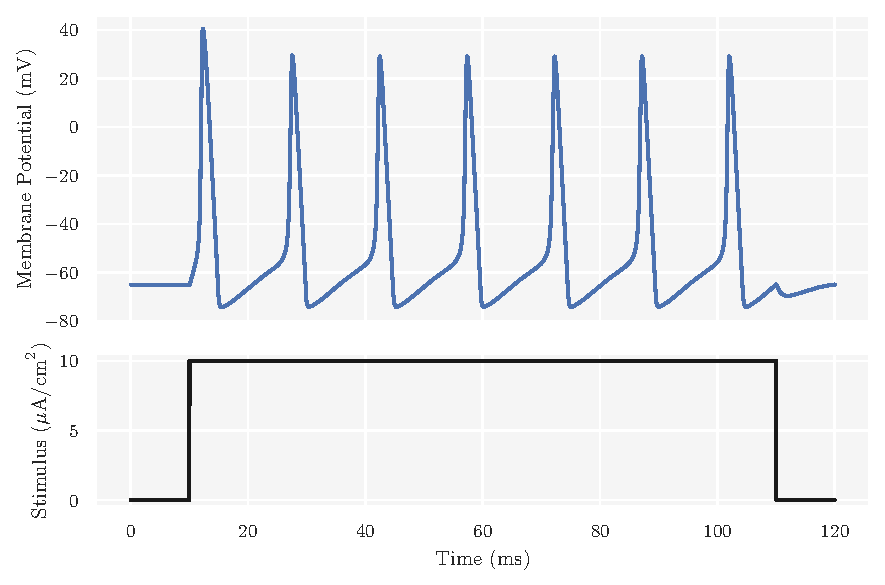
\includegraphics[scale=0.9]{hh_obs_data}
    \caption{Observed voltage trace of a current clamped neuron synthetically generated by the HH simulator simulated for $T = 120 \ms$ with time resolution $\Delta t=0.025 \ms$. The stimulus is a step current $I = 10 \, \mathrm{\mu A/cm}^2$ with onset and offset at $10 \ms$ and $110 \ms$, respectively. Here, the conductance parameters $\gbarK = 36 \gunit$ and $\gbarNa = 120 \gunit$. The present voltage trace being the observation, these conductance parameters are thus the ground truths for the subsequent analyses.}
    \label{fig:hh_obs_data}
\end{figure} 

From the voltage trace, we extract spike statistics by the computational algorithms outlined in \cref{sec:hh_feature_extract}. \autoref{fig:hh_stat_extraction} shows the locations in the voltage trace that form the basis of the spike statistic calculations. In fact, the annotations on the voltage trace are set automatically according to the positions found by the extraction algorithms. By the definitions of the different summary statistics provided in \cref{sec:spike_statistics}, we see that the extraction locations are placed correctly on the voltage trace. Consequently, the extraction algorithms seem to function as intended. 

\begin{figure}[!htb]
    \centering
    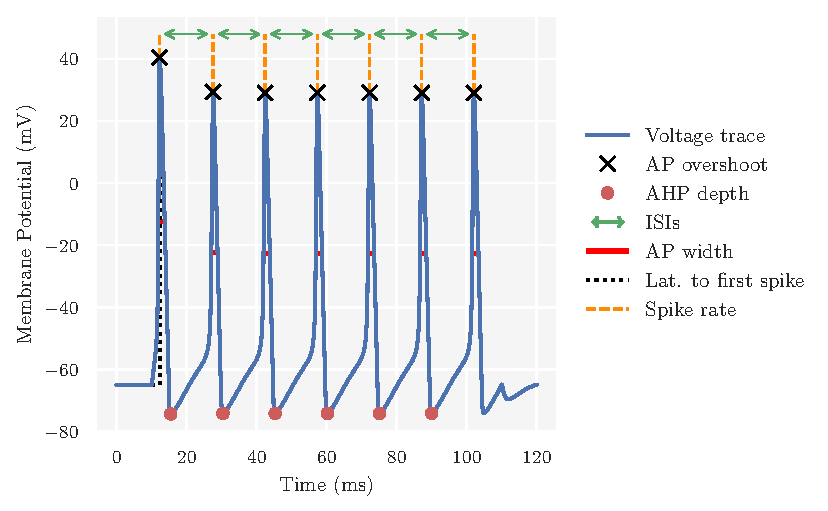
\includegraphics[scale=0.9]{hh_stat_extraction}
    \caption{Locations found by the feature extraction algorithms for spike statistic calculations on the observed voltage trace. The locations are annotated by different markers, with labels stated in the legend, which indicate the particular summary statistic calculation they are affiliated with.}
    \label{fig:hh_stat_extraction}
\end{figure} 

\autoref{tab:hh_obs_sumstats} summarizes the calculated summary statistics from the observed voltage trace; (i) \textit{spike rate}, calculated as the number of spikes divided by the duration of the stimulus; (ii) \textit{average AP overshoot}, calculated by averaging the absolute peak voltage of all APs; (iii) \textit{average AP width}, calculated by averaging the width of every AP at the midpoint between its onset and its peak; (iv) \textit{average AHP depth}, calculated by averaging all minima voltage throughs between two consecutive APs; (v) \textit{latency to first spike}, calculated as the time between stimulus onset and first AP peak; (vi) \textit{accommodation index}, which measures the local variance in ISIs and is calculated by \autoref{eq:accomm_index}. Comparing the values of the tabulated summary statistics with the information in \autoref{fig:hh_stat_extraction}, we find agreement. There are 7 spikes over the course of the stimulus duration of $100 \ms$, so the spike rate must be $0.07 \, \mathrm{mHz}$. Furthermore, the value of the average AP overshoot and width, as well as the average AHP depth, seems reasonable when compared with the voltage values at the extracted locations. A latency to first spike of about $2 \ms$ also matches what is seen in the voltage trace. There is practically no difference in length between two consecutive ISIs in the voltage trace, and the accommodation index should therefore reflect, as it does, the lack of variability. All in all, this indicates that also the summary statistic calculations are implemented correctly. 

\begin{table}[!htb]
  \caption{Observed voltage trace reduced to a set of summary statistics. See text for details on the statistics.  }
  %\footnotesize%
  \begin{center}
    \rowcolors{2}{gray!15}{white}
    \begin{tabular}{cc}
      \toprule
      \textbf{Summary statistic} & \textbf{Observed value} \\
      \midrule
      %Number of spikes &  7 \\
      Spike rate &  0.0700 mHz \\
      Average AP overshoot & 30.7316 mV  \\
      Average AP width &  2.0501 mV \\
      Average AHP depth & -74.2234 mV \\
      Latency to first spike & 2.3000 ms \\
      Accommodation index &  $2 \cdot 10^{-17}$ \\
      \bottomrule
    \end{tabular}
  \end{center}
  \label{tab:hh_obs_sumstats}
\end{table}

%================================================================
\subsection{Sensitivity Analysis}
%================================================================

Next, we carry out a sensitivity analysis of 

let us characterize the effects of parameter uncertainty on the output of the model in terms of the summary statistics.  

a sensitivity quantifies how much the uncertainty in the model output each model parameter is responsible for. 

While technically the informative priors could be classified as weakly-informative (as per the definition given in \cref{sec:coin_flipping}), we will refer to them as informative. 

\autoref{fig:hh_priors} Priors for HH

\begin{figure}[H]
    \centering
    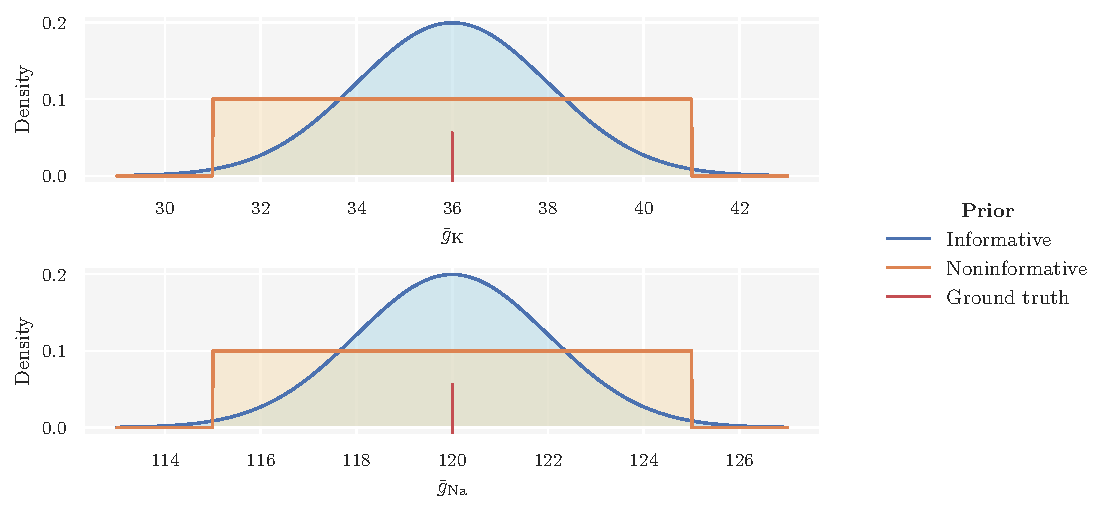
\includegraphics[scale=0.8]{hh_priors}
    \caption{caption}
    \label{fig:hh_priors}
\end{figure} 


\autoref{fig:hh_priorpred_sstats_normal} Summary statistics under the (informative) prior predictive distribution (draw 2000 samples, dropna -> left with 1881 samples, but here we only plot a subset of 470 samples)

\begin{figure}[H]
    \centering
    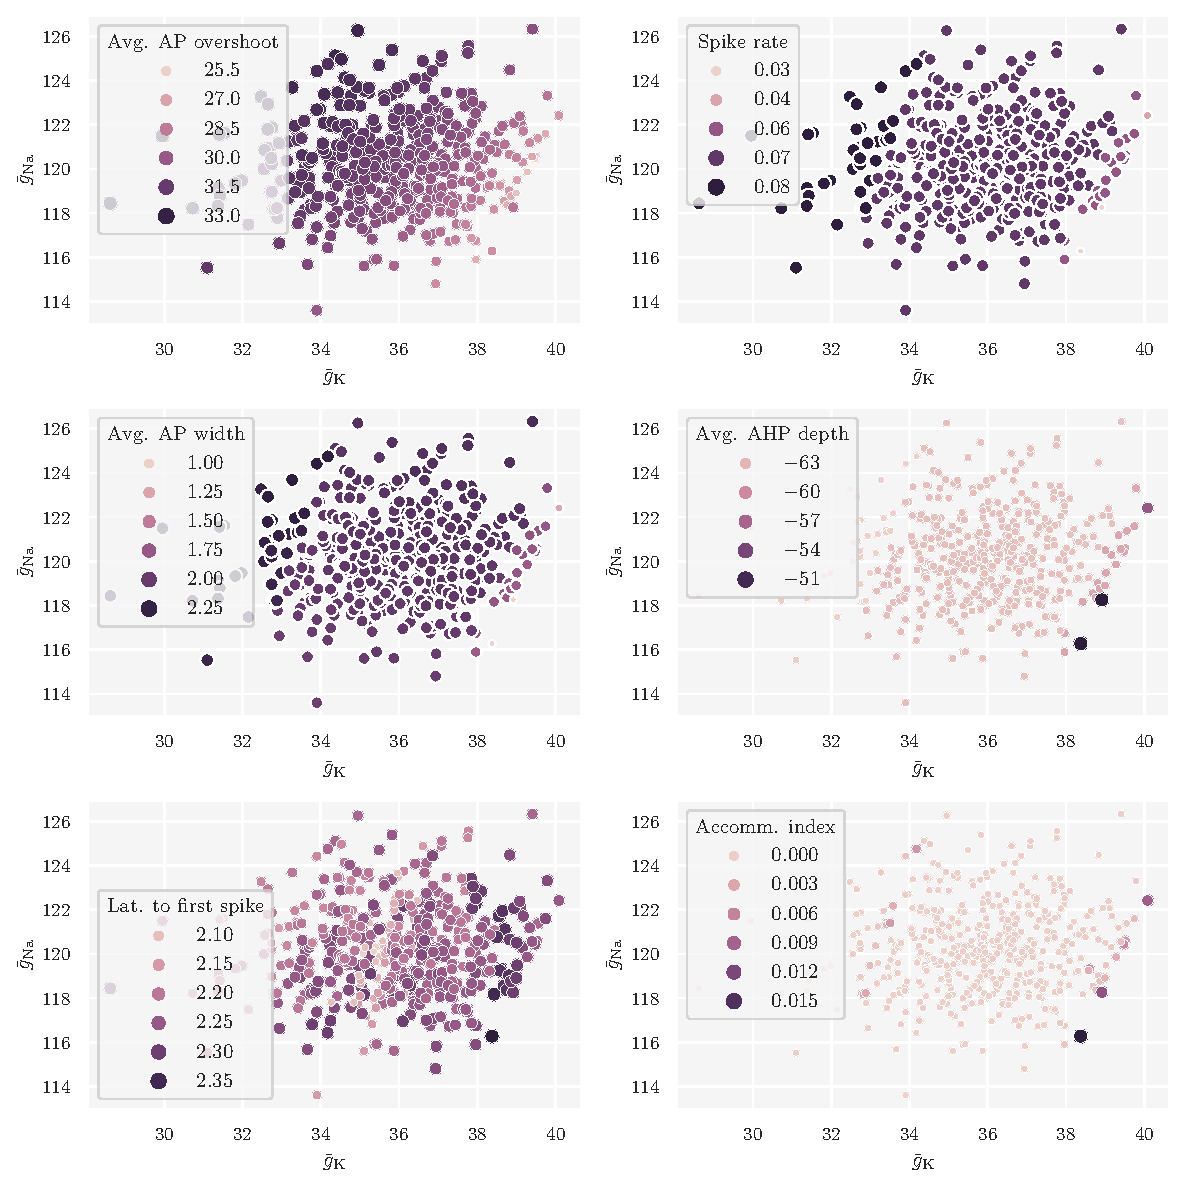
\includegraphics[scale=0.8]{hh_priorpred_sstats_normal}
    \caption{caption}
    \label{fig:hh_priorpred_sstats_normal}
\end{figure} 


\autoref{fig:hh_weights_normal} sum stats correlation (pearson) and weights

% subfigure
\begin{figure}[H]
\centering
\subfloat[]{{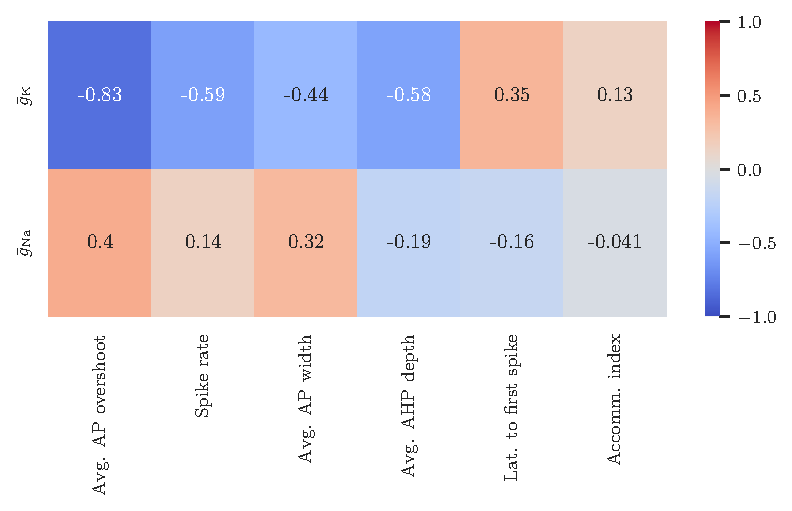
\includegraphics[scale=0.7]{hh_priorpred_corr_normal}}}
\qquad
\subfloat[]{{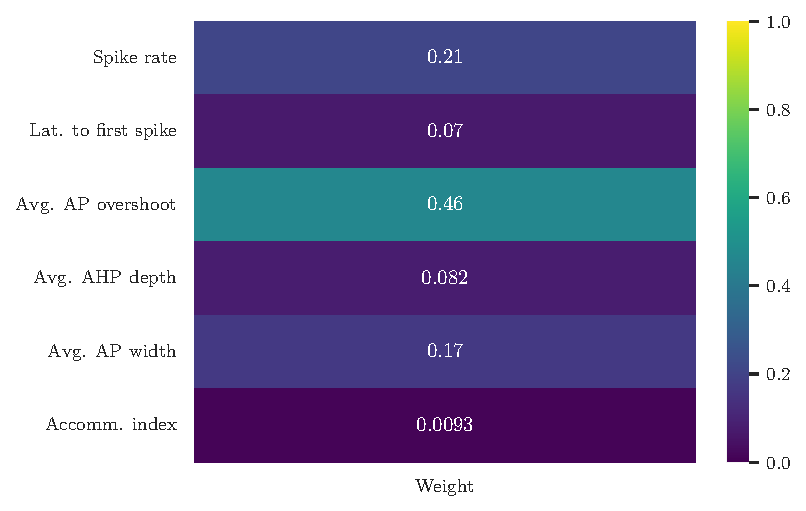
\includegraphics[scale=0.7]{hh_priorpred_weights_normal}}}
\caption{\textbf{(a)} sum stats correlation. \textbf{(b)} sum stats weights from corr coef
}
\label{fig:hh_weights_normal}
\end{figure}


Perhaps unsurprisingly, since the prior distribution does not alter the inherent relationship between the quantities, we obtain the same weights from the summary statistics generated under the noninformative prior predictive distribution. The same results as above for the noninformative prior can be found in ... ref appendix A section ...




%%
%% BRUNEL
%%

%================================================================
\chapter{Inference on Brunel}\label{chap:res_brunel}
%================================================================ 

Chapter Inference on the Brunel model
- observed data 
- priors
- prior predictive sum stats 
- rej-abc (original) posteriors 
- reg adj posteriors
- ppc 
- sbi


%%
%%
%%
%%
%%

%================================================================
%\chapter{Analysis of the Hodgkin-Huxley Model}
\chapter{Analysis of the Neuroscientific Models}
%================================================================

% chapter: Inference on the Hodgkin-Huxley Model 
% chapter: Inference on the Brunel Model

%================================================================
\section{The Hodgkin-Huxley Model}
%================================================================




\subsection{Noisy HH Data}

\begin{figure}[H]
    \centering
    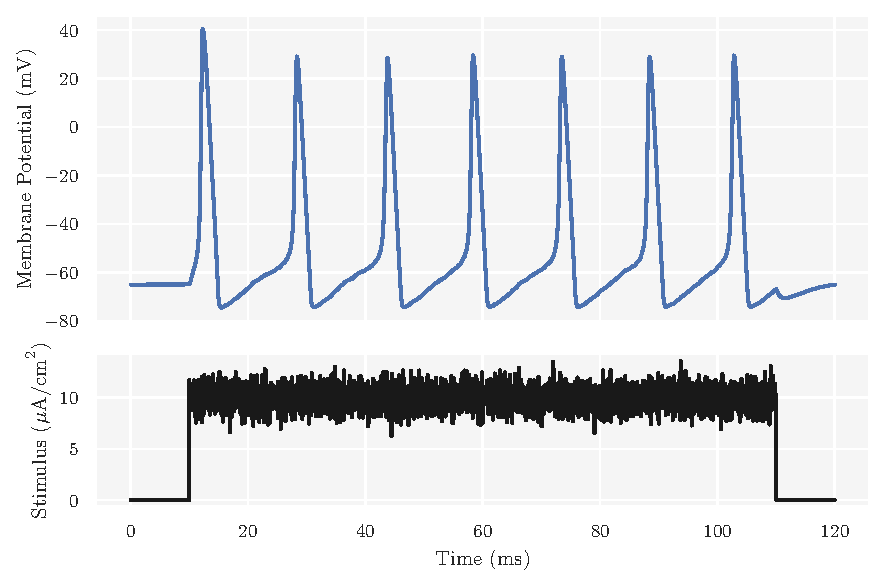
\includegraphics[scale=0.9]{hh_noisy_data}
    \caption{caption}
    \label{fig:fig1}
\end{figure} 


% Alternating row colors
\begin{table}[H]
  \caption{Generic table with alternating rows and different sized rulers. The number of spikes is not used as a summary statistic in and of itself, but is included to show that the statistic extraction indeed finds all spikes.}
  %\footnotesize%
  \begin{center}
    \rowcolors{2}{gray!15}{white}
    \begin{tabular}{cc}
      \toprule
      \textbf{Summary statistic} & \textbf{Observed value} \\
      \midrule
      Number of spikes &  7 \\
      Spike rate &  0.0700 mHz \\
      Average AP overshoot & 30.7223 mV  \\
      Average AP width & 2.0679 mV \\
      Average AHP depth & -74.3394 mV \\
      Latency to first spike & 2.2750 ms \\
      Accommodation index &  -0.0067 \\
      \bottomrule
    \end{tabular}
  \end{center}
  \label{tab:hh_noisy_sumstats}
\end{table}



----

observed data w/o noise 

feature extraction 

plot features 

compute weights (plot correlation matrix) 

plot priors (informative, noninformative)


---

create the observed data

summary statistics of observation 

summary statistics from prior predictive

weights

(observed data with noise; same as above)

%================================================================
\section{The Brunel Network Model}
%================================================================

create the observed data

summary statistics of observation 

summary statistics from prior predictive

weights


%================================================================
\chapter{Parameter Identification with REJ-ABC}
%================================================================

%================================================================
\section{Rejection ABC Posteriors on Conductance Parameters}
%================================================================

show how Hodgkin–Huxley model is more tightly constrained by increasing numbers of data features

We also inferred HH parameters for 8 in vitro recordings from the Allen Cell Types database using the same current-clamp stimulation protocol as in our model [60, 70] (Fig. 4F, Supplementary Fig. 8). In each case, simulations based on the SNPE-inferred posterior closely resembled the original data (Fig. 4F). We note that while inferred parameters differed across recordings, some parameters (the spike threshold, the density of sodium channels, the membrane reversal potential and the density of potassium channels) were consistently more strongly constrained than others (the intrinsic neural noise, the adaptation time constant, the density of slow voltage-dependent channels and the leak conductance) (Supplementary Fig. 8). Overall, these results suggest that the electrophysiological responses measured by this current-clamp protocol can be approximated by a single-compartment HH model, and that SNPE can identify the admissible parameters.

%================================================================
\subsection{ABC Settings for Identification of Hodgkin-Huxley Parameters}
%================================================================

RMSE averaged over 10 posteriors for each quantile value. 1000 posterior samples in each posterior. 

\begin{figure}[H]
    \centering
    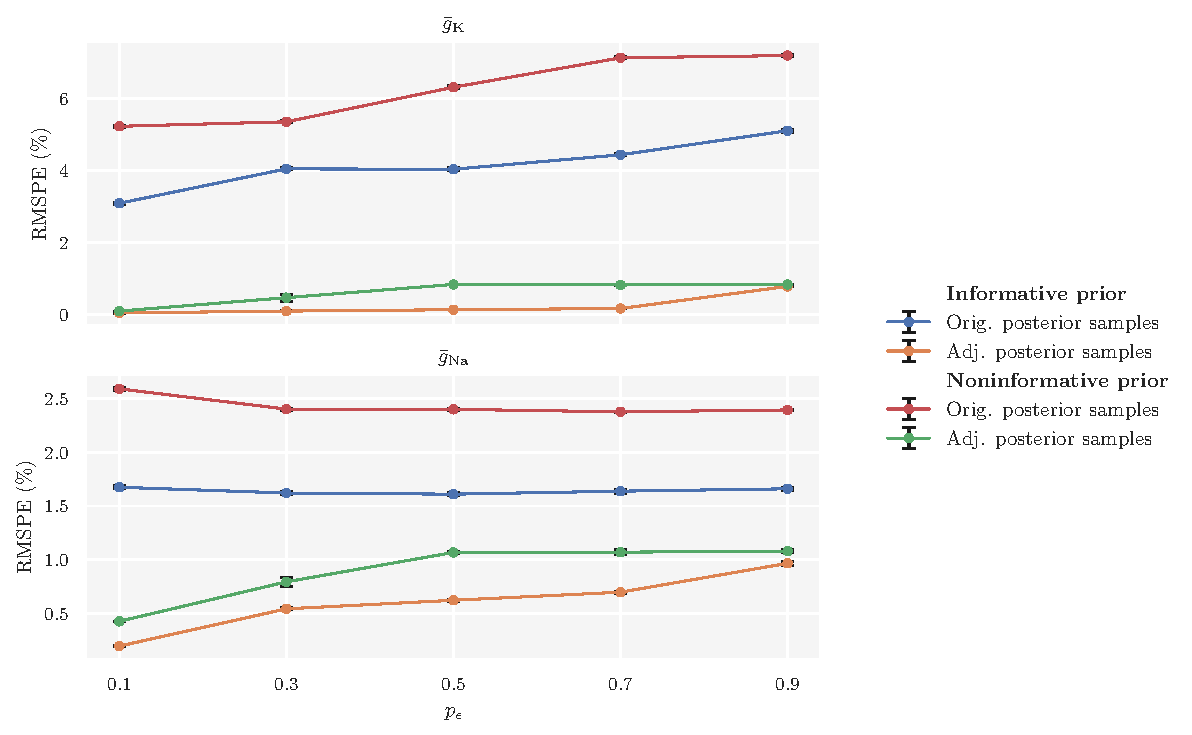
\includegraphics[scale=0.8]{RMSPE_vs_quantile}
    \caption{caption}
    \label{fig:fig1}
\end{figure} 

0.4 quantile, compromise between accuracy and computational demands (see fig runtime in appendix)

Number of summary statistics

\begin{figure}[H]
    \centering
    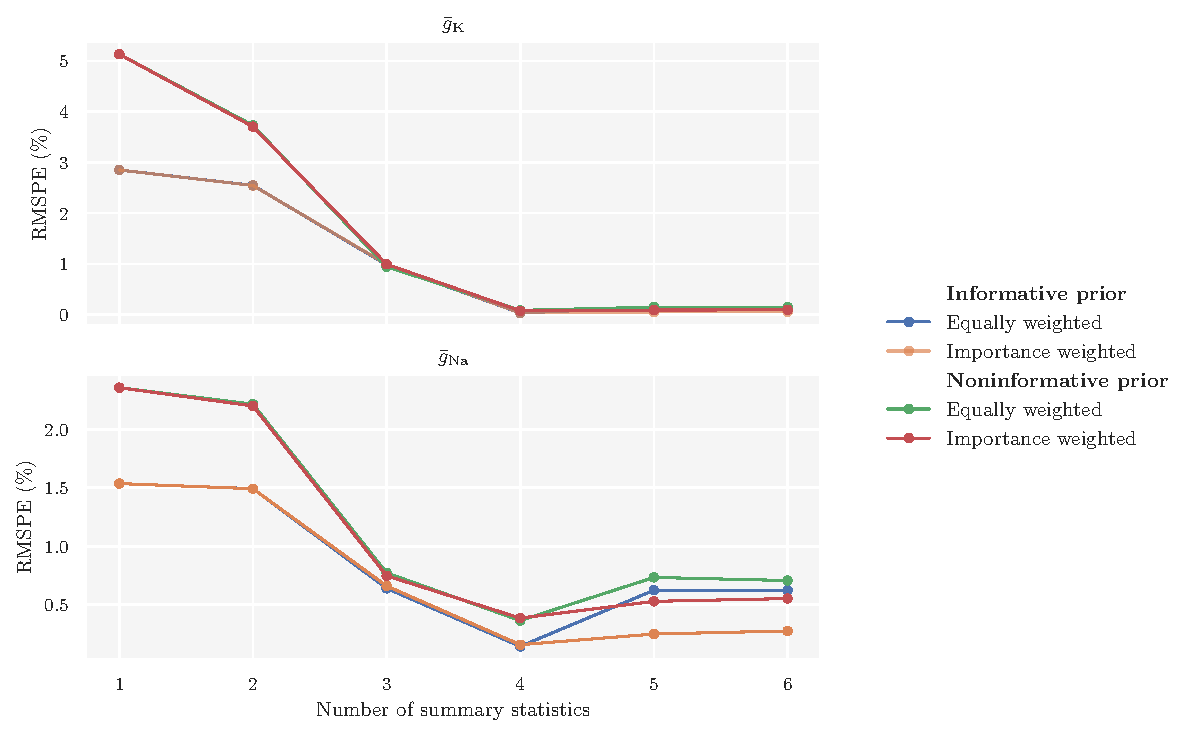
\includegraphics[scale=0.8]{RMSPE_vs_n_sumstats}
    \caption{caption}
    \label{fig:fig1}
\end{figure} 


\subsection{Summarizing Posteriors, informative priors}

Posteriors with original samples, informative prior

\begin{figure}[H]
    \centering
    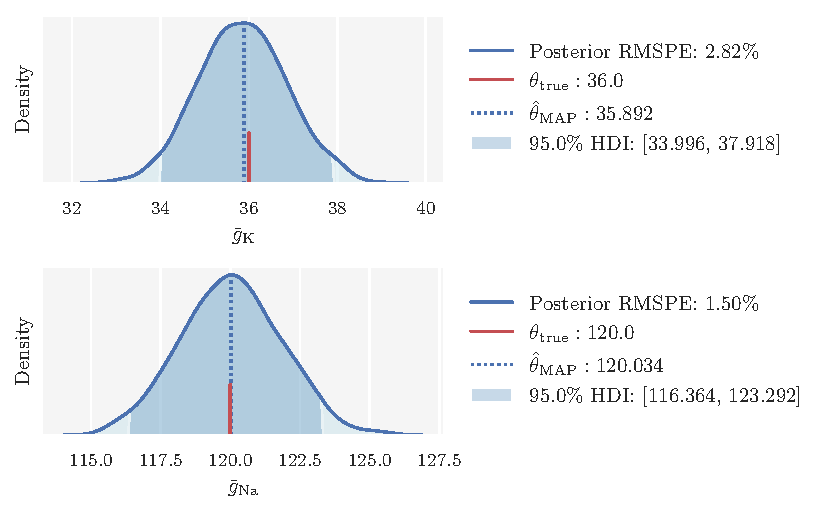
\includegraphics[scale=1]{hh_posterior_org_normal}
    \caption{caption}
    \label{fig:fig1}
\end{figure}

Make subfig with corr and joint

Correlation 

\begin{figure}[H]
    \centering
    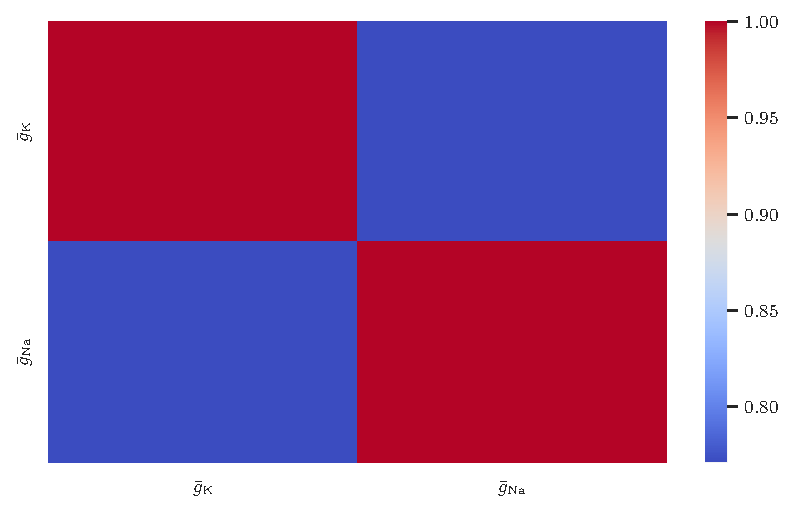
\includegraphics[scale=0.8]{hh_corr_org_normal}
    \caption{caption}
    \label{fig:fig1}
\end{figure}

Joint posterior 

\begin{figure}[H]
    \centering
    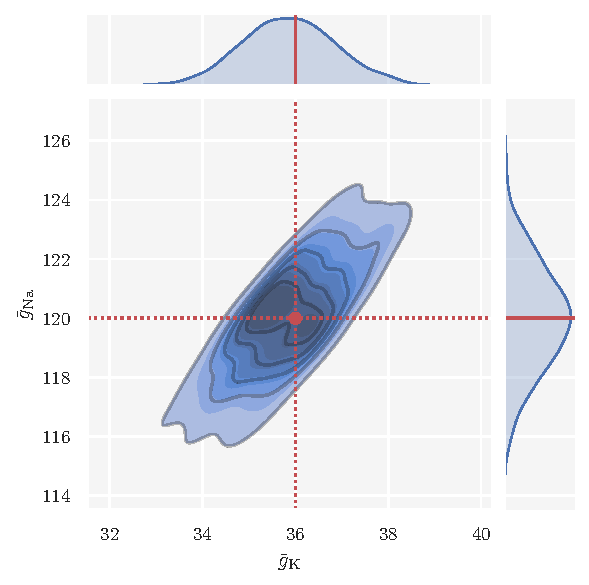
\includegraphics[scale=1.0]{hh_joint_posterior_org_normal}
    \caption{caption}
    \label{fig:fig1}
\end{figure}

Posteriors, reg adjusted samples, informative prior

\begin{figure}[H]
    \centering
    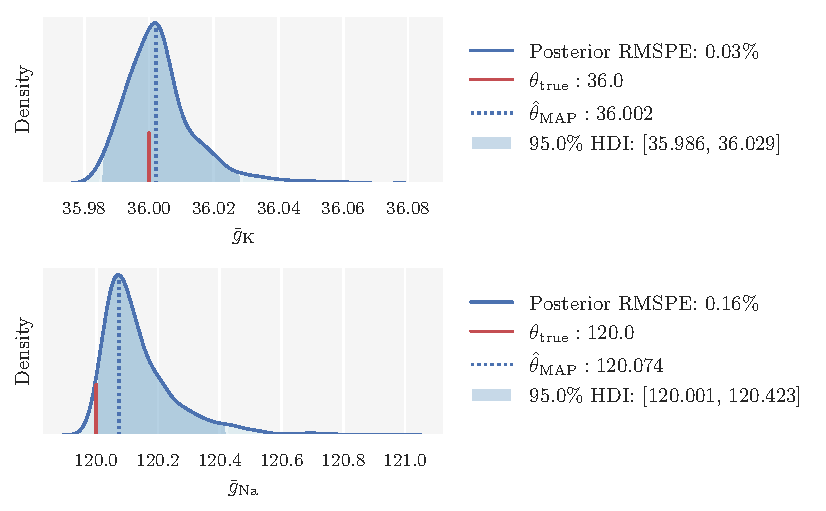
\includegraphics[scale=1.0]{hh_posterior_reg_normal}
    \caption{caption}
    \label{fig:fig1}
\end{figure}

PPC reg adjusted posterior predictive 

\begin{figure}[H]
    \centering
    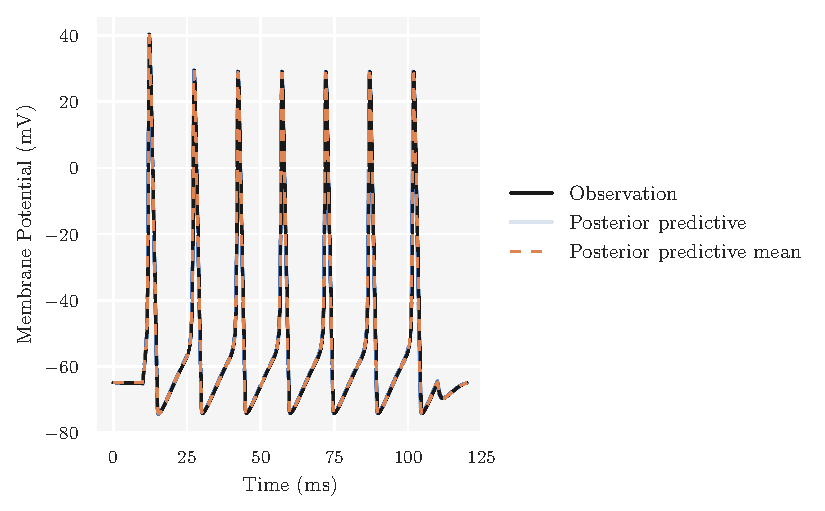
\includegraphics[scale=1.0]{hh_postpred_reg_normal}
    \caption{caption}
    \label{fig:fig1}
\end{figure}


As can be seen, the samples from the inferred posterior lead to simulations that closely resemble the observed data, confirming that Rej-ABC did a good job at capturing the observed data in this simple case.

\subsection{Summarizing Posteriors, noninformative priors}

posterior, original, noninfo prior

\begin{figure}[H]
    \centering
    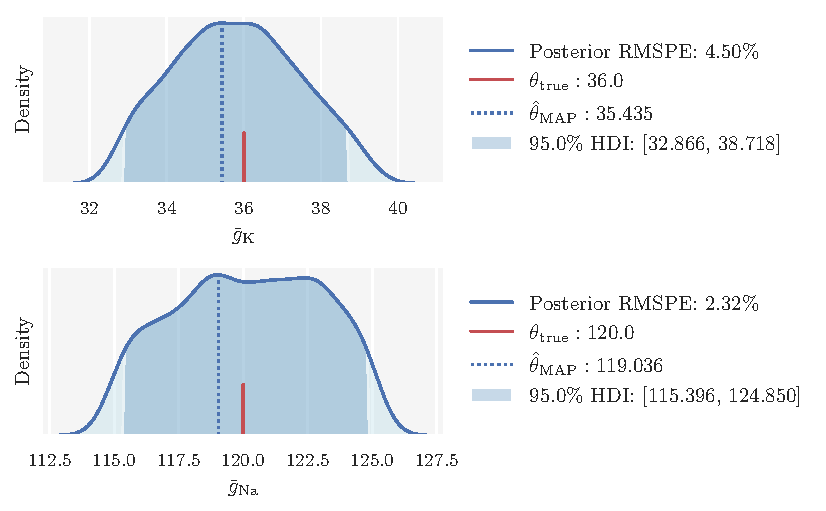
\includegraphics[scale=1.0]{hh_posterior_org_uniform}
    \caption{caption}
    \label{fig:fig1}
\end{figure}

Adjusted posterior, noninformative prior

\begin{figure}[H]
    \centering
    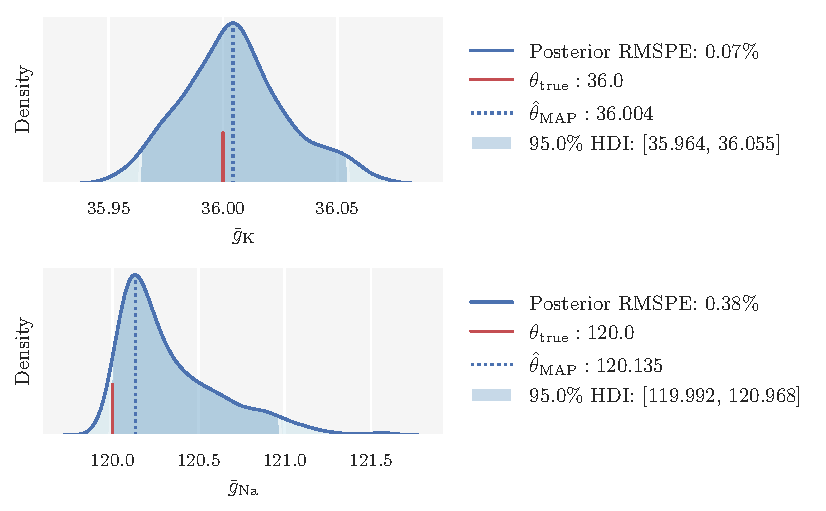
\includegraphics[scale=1.0]{hh_posterior_reg_uniform}
    \caption{caption}
    \label{fig:fig1}
\end{figure} 

PPC adjusted posterior 

\begin{figure}[H]
    \centering
    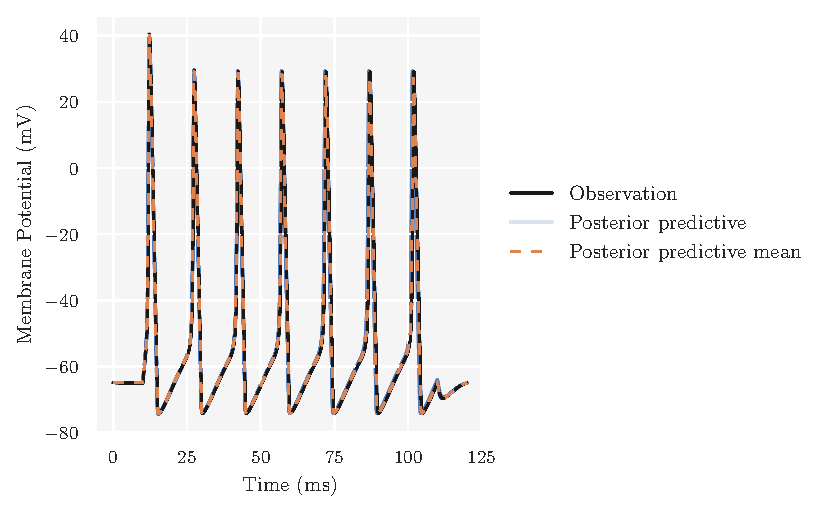
\includegraphics[scale=1.0]{hh_postpred_reg_uniform}
    \caption{caption}
    \label{fig:fig1}
\end{figure}

\subsection{Noisy observation} 

original posterior on noisy observed data

\begin{figure}[H]
    \centering
    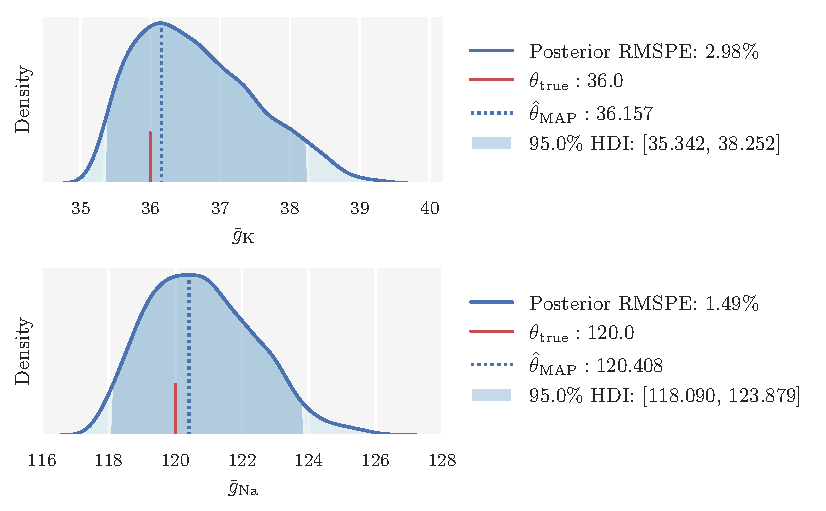
\includegraphics[scale=1.0]{hh_posterior_org_noisy}
    \caption{caption}
    \label{fig:fig1}
\end{figure} 

adjusted posterior on noisy observed data

\begin{figure}[H]
    \centering
    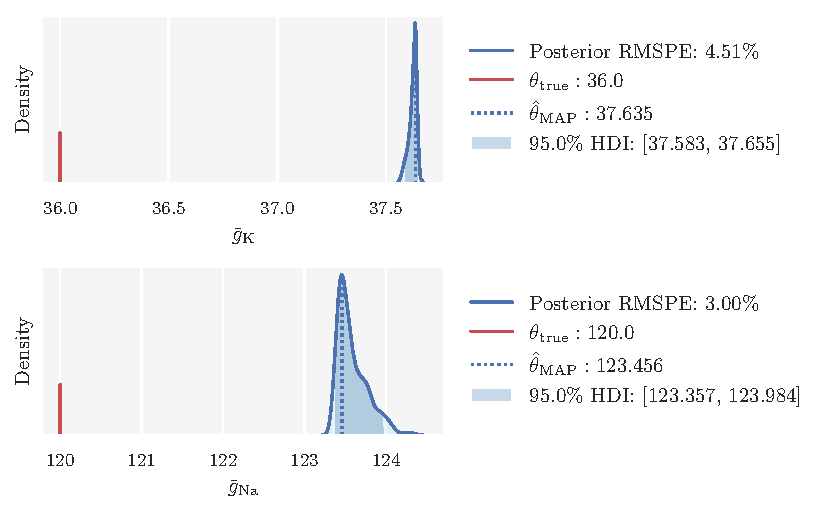
\includegraphics[scale=1.0]{hh_posterior_reg_noisy}
    \caption{caption}
    \label{fig:fig1}
\end{figure} 

ppc with reg adjusted posterior samples (100 posterior samples)


\begin{figure}[H]
    \centering
    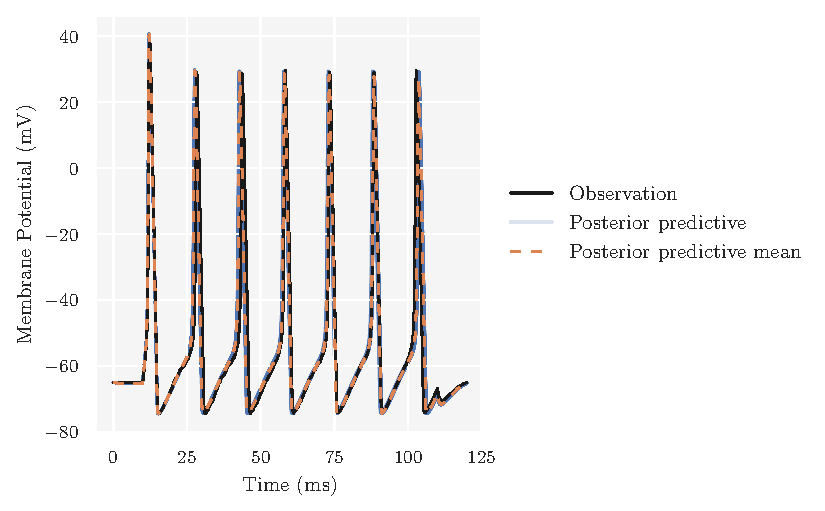
\includegraphics[scale=1.0]{hh_postpred_reg_noisy}
    \caption{caption}
    \label{fig:fig1}
\end{figure}

%================================================================
%\section{ABC Settings for Identification of Brunel Network Parameters}
%================================================================

%================================================================
%\section{Rejection ABC Posteriors on Synaptic Weight Parameters}
%================================================================

%================================================================
\chapter{Brunel ABC Results}
%================================================================

Brunel 

\section{Observation}

observed spiketrain 

\begin{figure}[H]
    \centering
    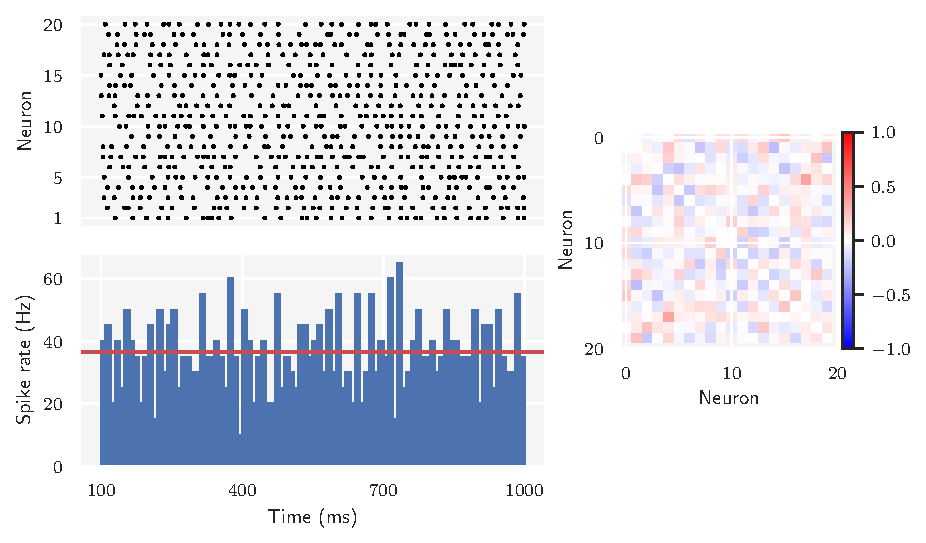
\includegraphics[scale=1.0]{brunel_ai_observation}
    \caption{caption}
    \label{fig:fig1}
\end{figure}

sum stats

% Alternating row colors
\begin{table}[H]
  \caption{AI state observed sum stats}
  %\footnotesize%
  \begin{center}
    \rowcolors{2}{gray!15}{white}
    \begin{tabular}{cc}
      \toprule
      \textbf{Summary statistic} & \textbf{Observed value} \\
      \midrule
      Mean firing rate &  0.0366 kHz \\
      Mean CV &  0.4250  \\
      Fano factor & 0.2341  \\
      \bottomrule
    \end{tabular}
  \end{center}
  \label{tab:hh_noisy_sumstats}
\end{table}

correlation (pearson) coefficient matrix

\begin{figure}[H]
    \centering
    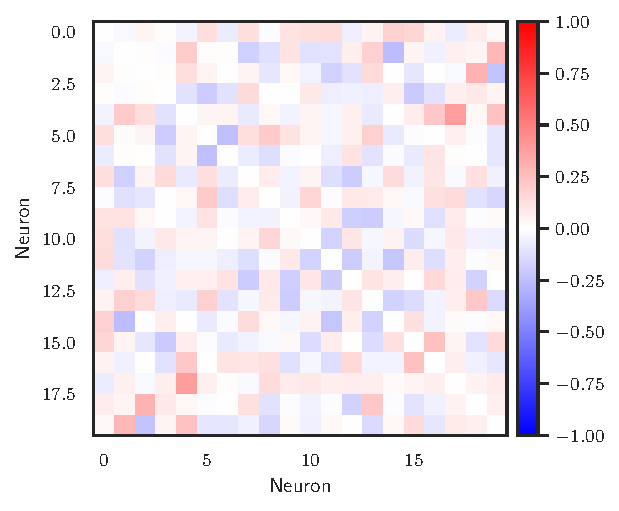
\includegraphics[scale=1.0]{brunel_obs_corr}
    \caption{caption}
    \label{fig:fig1}
\end{figure}

\section{prior pred}

priors

\begin{figure}[H]
    \centering
    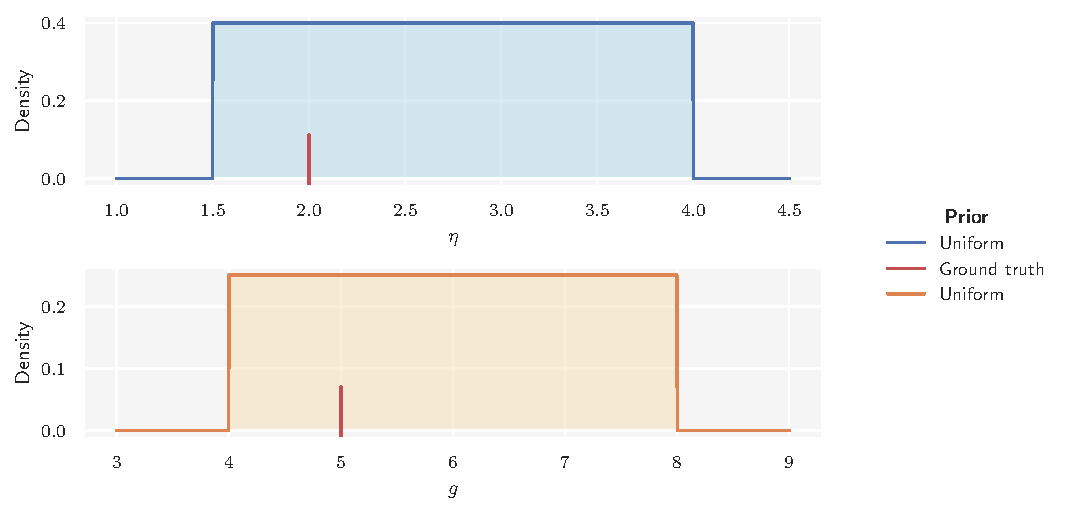
\includegraphics[scale=0.8]{brunel_priors}
    \caption{caption}
    \label{fig:fig1}
\end{figure}

sum stats scatter (500 samples)

\begin{figure}[H]
    \centering
    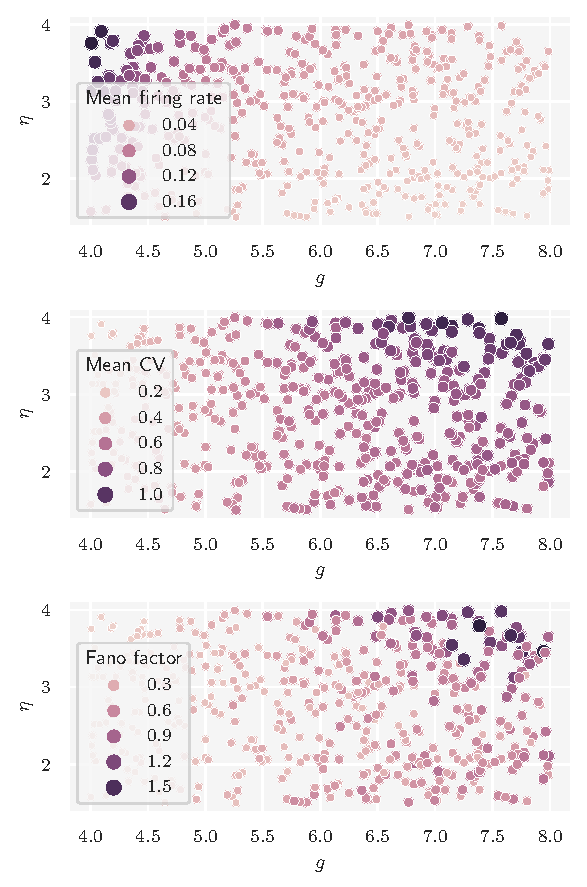
\includegraphics[scale=1.0]{brunel_sum_stats}
    \caption{caption}
    \label{fig:fig1}
\end{figure}


sum stats correlation and weights

% subfigure
\begin{figure}[H]
\centering
\subfloat[]{{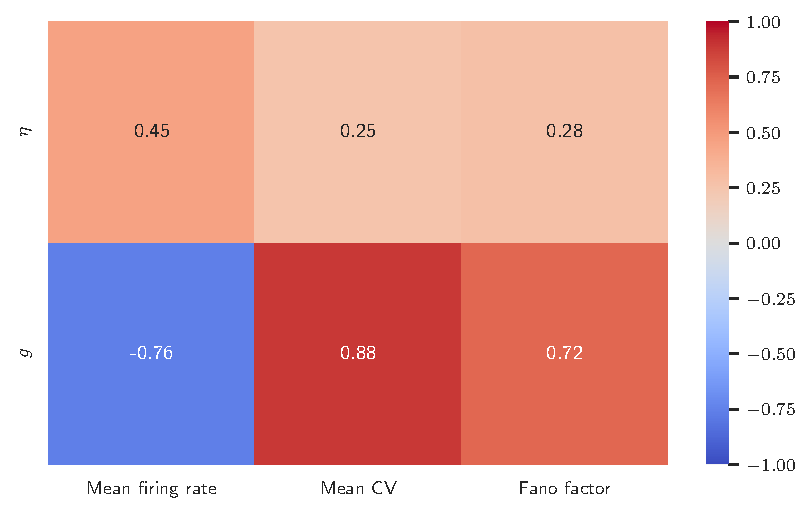
\includegraphics[scale=0.7]{brunel_sum_stats_corr}}}
\qquad
\subfloat[]{{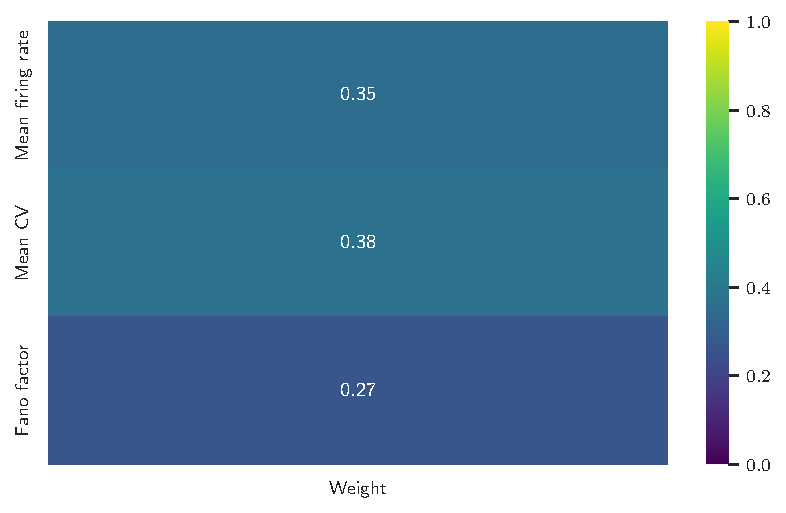
\includegraphics[scale=0.7]{brunel_sum_stats_weights}}}
\caption{\textbf{(a)} sum stats correlation. \textbf{(b)} sum stats weights
}
\label{fig:fig1}
\end{figure}

corr coefs of these particular summary statistics indicate that the AI state is most sensitive to the relative strength of inhibitory synapses $g$. Thus, we expect the summary statistics to constrain the $g$ parameter better.


\section{Posteriors} 

Ran 2000 simulations of the model with different parameters drawn from the priors. RMSPE vs quantile: 

\begin{figure}[H]
    \centering
    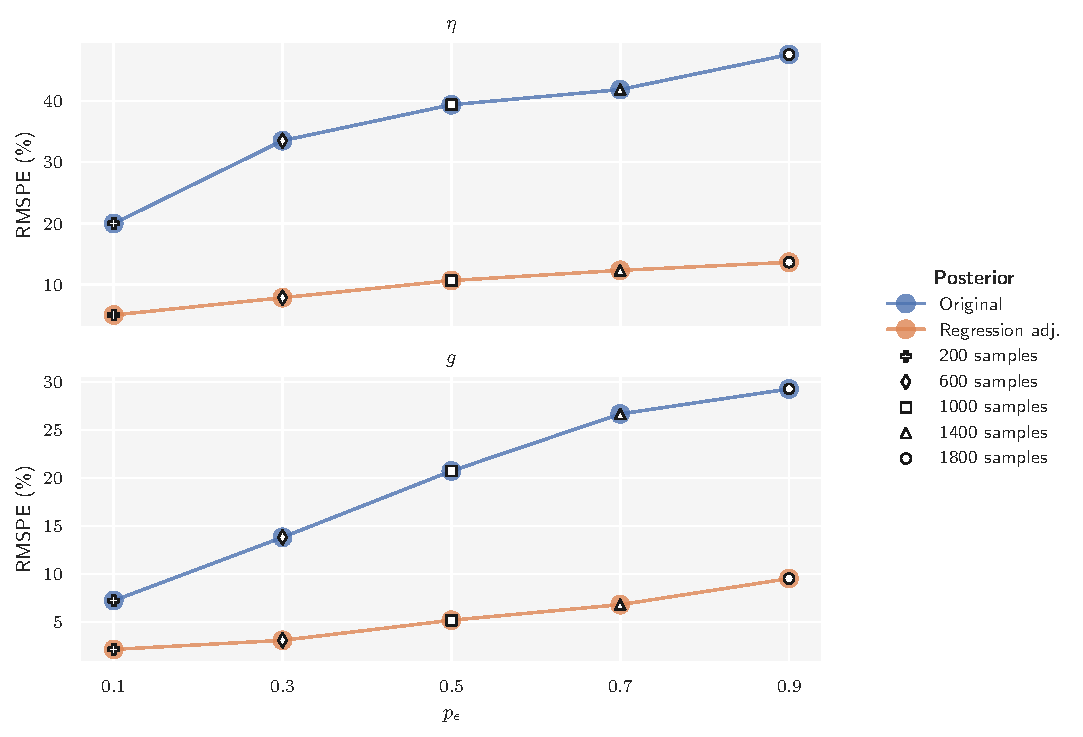
\includegraphics[scale=0.8]{brunel_quantile_rmspe}
    \caption{caption}
    \label{fig:fig1}
\end{figure}

Use 0.3-quantile, compromise between accuracy and number of samples in the posterior

original posterior

\begin{figure}[H]
    \centering
    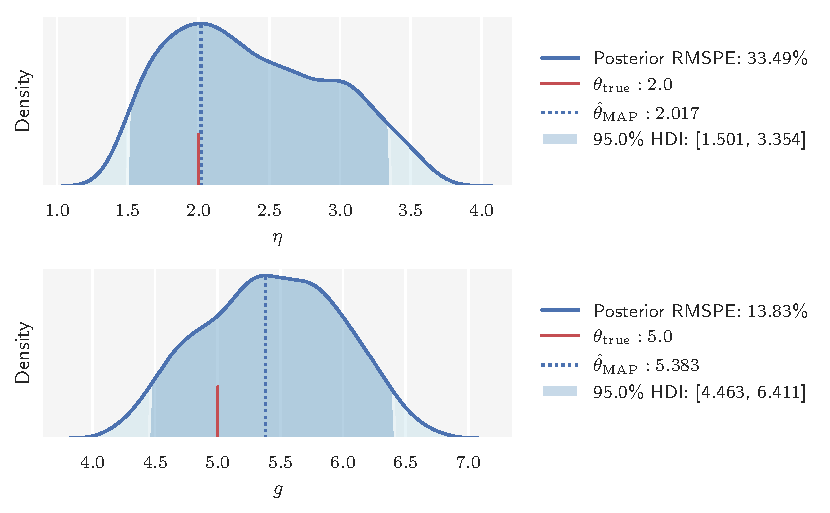
\includegraphics[scale=1.0]{brunel_posterior_org}
    \caption{caption}
    \label{fig:fig1}
\end{figure}

reg adjusted posterior

\begin{figure}[H]
    \centering
    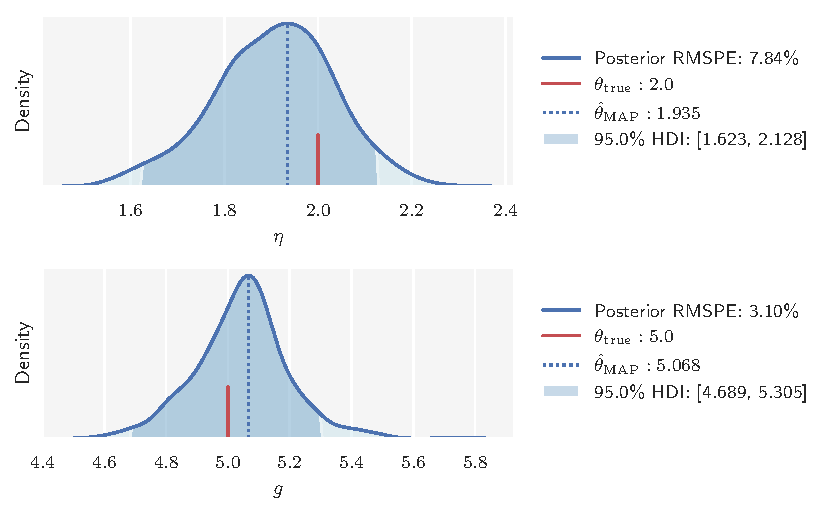
\includegraphics[scale=1.0]{brunel_posterior_reg}
    \caption{caption}
    \label{fig:fig1}
\end{figure}


joint posterior (reg adjusted)

\begin{figure}[H]
    \centering
    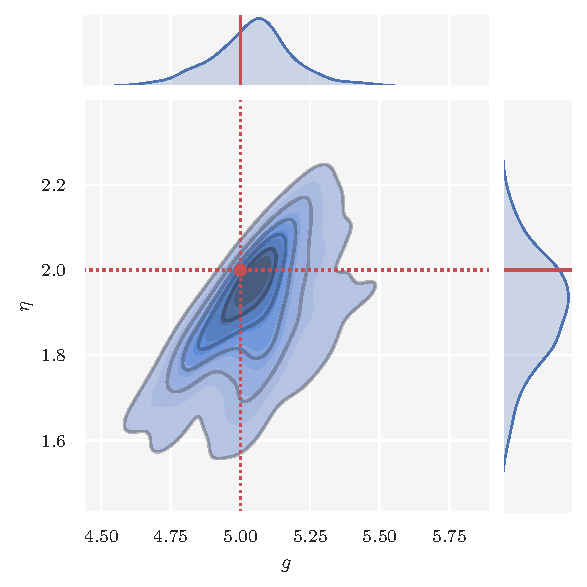
\includegraphics[scale=1.0]{brunel_joint_posterior_reg}
    \caption{caption}
    \label{fig:fig1}
\end{figure}

posterior predictive checks with reg adjusted samples, 50 samples from posterior pred

\begin{figure}[H]
    \centering
    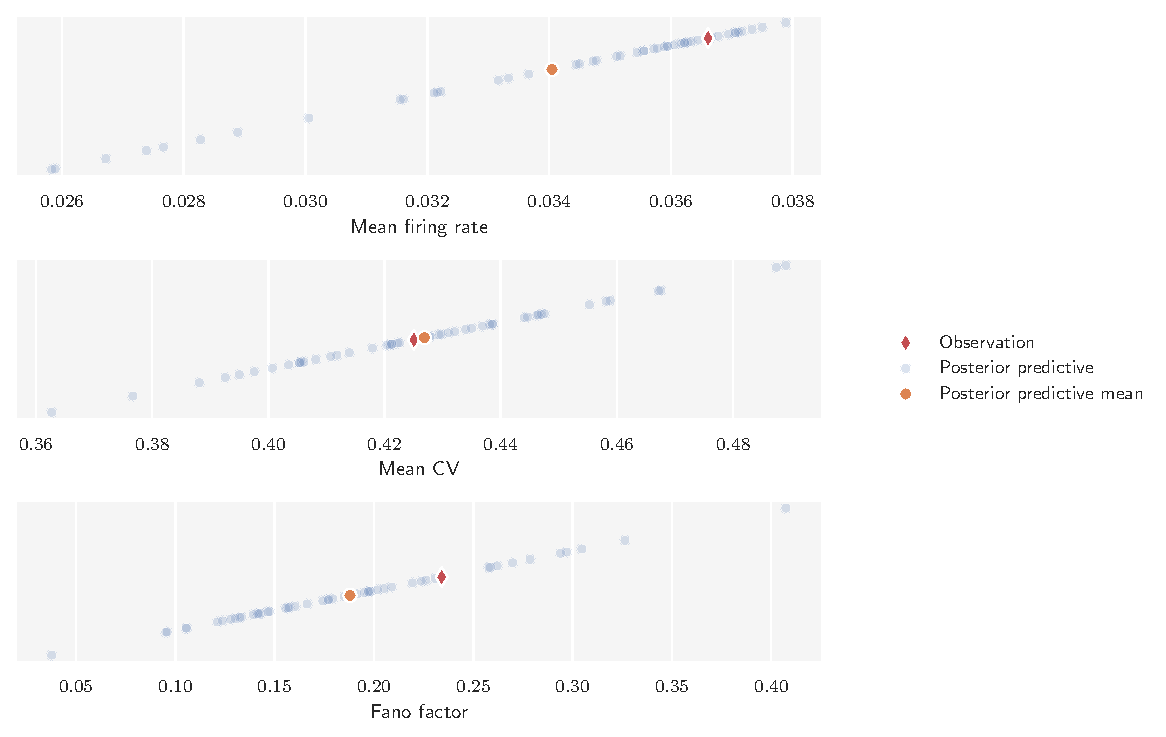
\includegraphics[scale=0.8]{brunel_post_pred}
    \caption{caption}
    \label{fig:fig1}
\end{figure}

The pairwise Pearson's correlation coefficient is a measure of how synchronous the spiking of a network is. This correlation coefficient measures the correlation between the spike trains of two neurons in the network. In Figure X we examine how this correlation depends on parameter uncertainties by plotting the mean and standard deviation for the pairwise Pearson's correlation coefficient in the AI state.

% subfigure
\begin{figure}[H]
\centering
\subfloat[]{{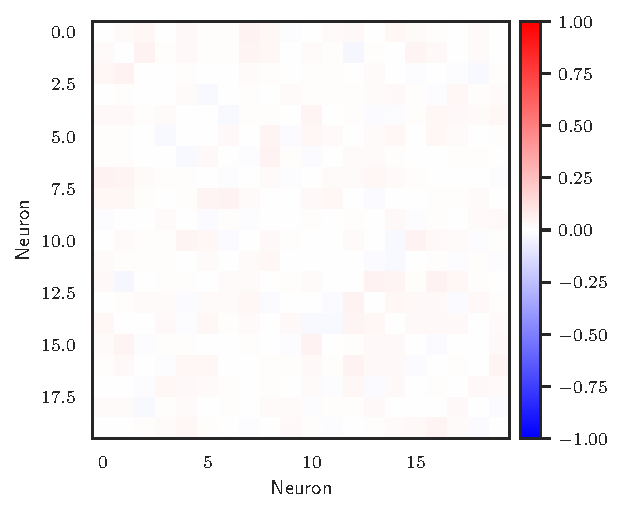
\includegraphics[scale=0.6]{brunel_pred_corr}}}
\qquad
\subfloat[]{{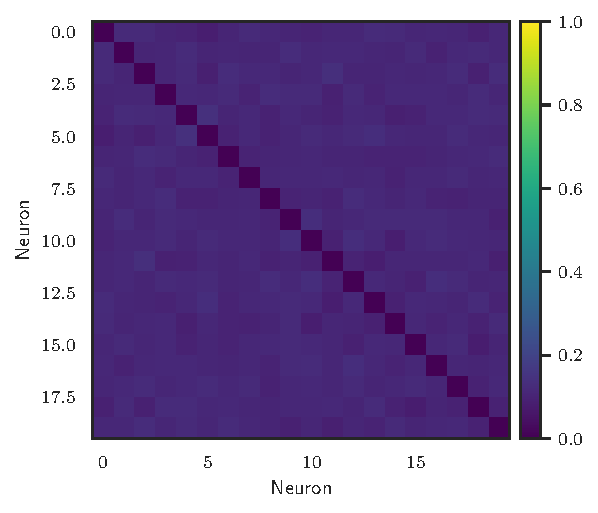
\includegraphics[scale=0.6]{brunel_pred_corr_std}}}
\caption{\textbf{(a)} mean correlation coefficient matrix. \textbf{(b)} standard deviation
}
\label{fig:fig1}
\end{figure}


%================================================================
\section{HH SBI Results}
%================================================================

same observed data as for clean hh

Posterior:

\begin{figure}[H]
    \centering
    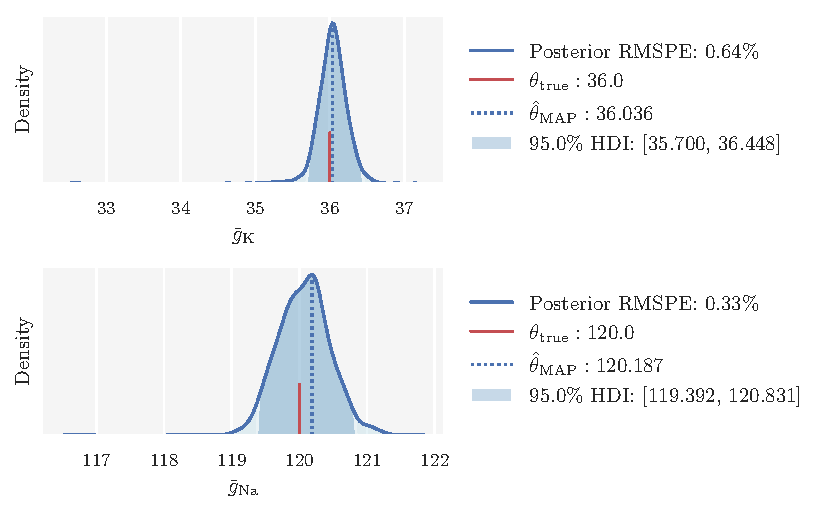
\includegraphics[scale=0.8]{hh_post_sbi}
    \caption{caption}
    \label{fig:fig1}
\end{figure}

PPC

\begin{figure}[H]
    \centering
    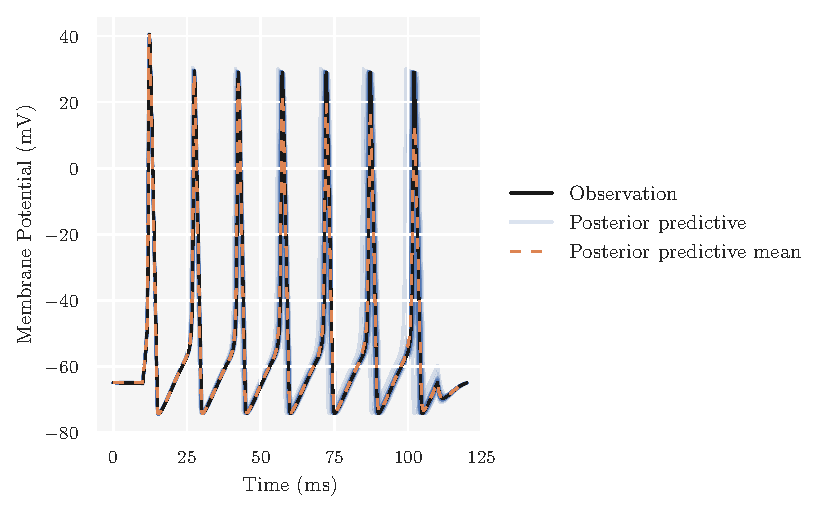
\includegraphics[scale=0.8]{hh_post_pred_sbi}
    \caption{caption}
    \label{fig:fig1}
\end{figure}

see that the wider posterior has an effect on recreating the observed data, this is not present in rej-abc reg adjust posterior due to it being more narrow


%================================================================
\section{Brunel SBI Results}
%================================================================

%================================================================
\subsection{AI state} 
%================================================================



0.037222	0.401465	0.145315

Posterior:

\begin{figure}[H]
    \centering
    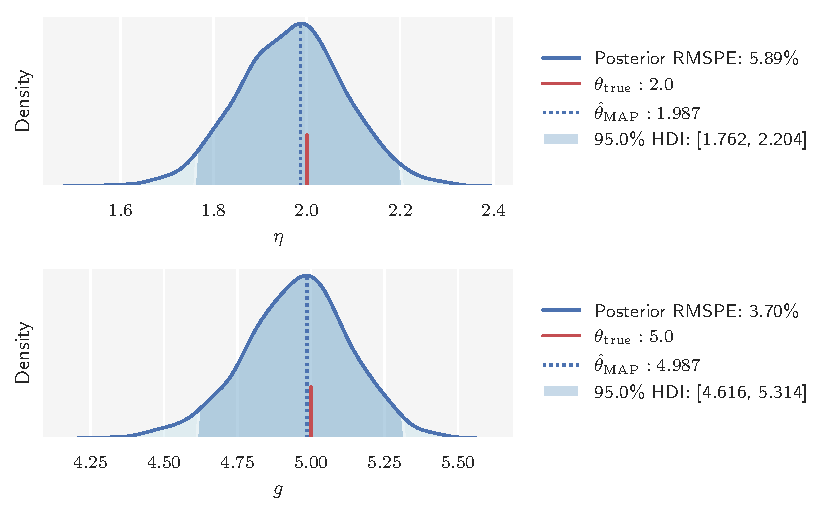
\includegraphics[scale=0.8]{brunel_post_ai_sbi}
    \caption{caption}
    \label{fig:fig1}
\end{figure}

ppc 

\begin{figure}[H]
    \centering
    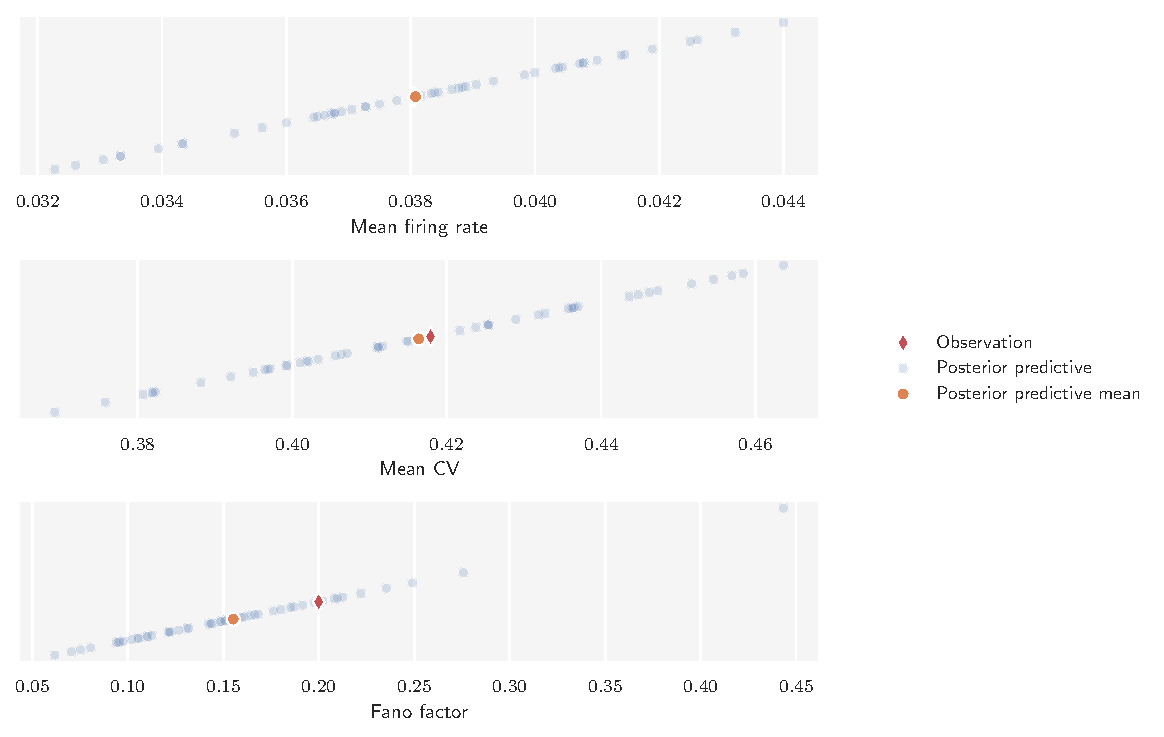
\includegraphics[scale=0.8]{brunel_post_pred_ai_sbi}
    \caption{caption}
    \label{fig:fig1}
\end{figure}

corr 

\begin{figure}[H]
    \centering
    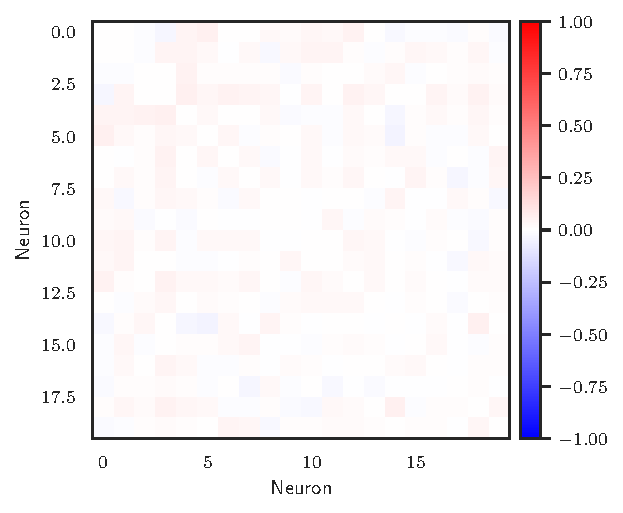
\includegraphics[scale=0.8]{brunel_pred_corr_sbi_ai}
    \caption{caption}
    \label{fig:fig1}
\end{figure}

corr std

\begin{figure}[H]
    \centering
    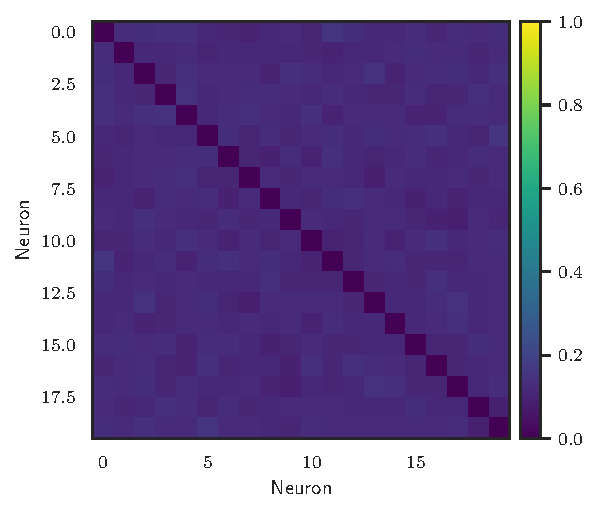
\includegraphics[scale=0.8]{brunel_pred_corr_std_ai_sbi}
    \caption{caption}
    \label{fig:fig1}
\end{figure}

%================================================================
\subsection{SR state}
%================================================================

SR observation

\begin{figure}[H]
    \centering
    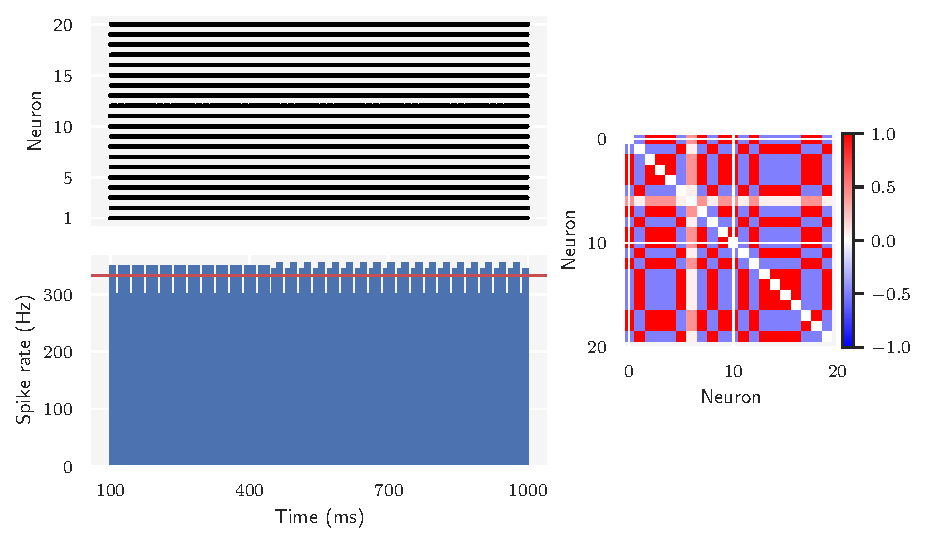
\includegraphics[scale=1.0]{brunel_sr_observation}
    \caption{caption}
    \label{fig:fig1}
\end{figure}

Recorded spike trains from the Brunel network and observed the following summary statistics:

\begin{table}[H]
  \caption{SR state observation.}
  %\footnotesize%
  \begin{center}
    \rowcolors{2}{gray!15}{white}
    \begin{tabular}{cc}
      \toprule
      \textbf{Summary statistic} & \textbf{Observed value} \\
      \midrule
      Mean firing rate &  0.3333 kHz \\
      Mean CV &  0.0121  \\
      Fano factor & 0.007  \\
      \bottomrule
    \end{tabular}
  \end{center}
  \label{tab:hh_noisy_sumstats}
\end{table}

Posterior:

\begin{figure}[H]
    \centering
    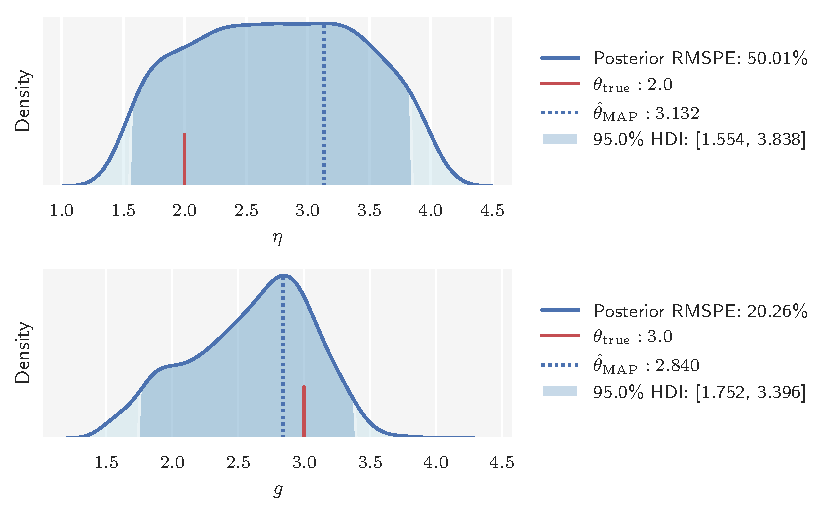
\includegraphics[scale=0.8]{brunel_post_sr_sbi}
    \caption{caption}
    \label{fig:fig1}
\end{figure}

ppc 

\begin{figure}[H]
    \centering
    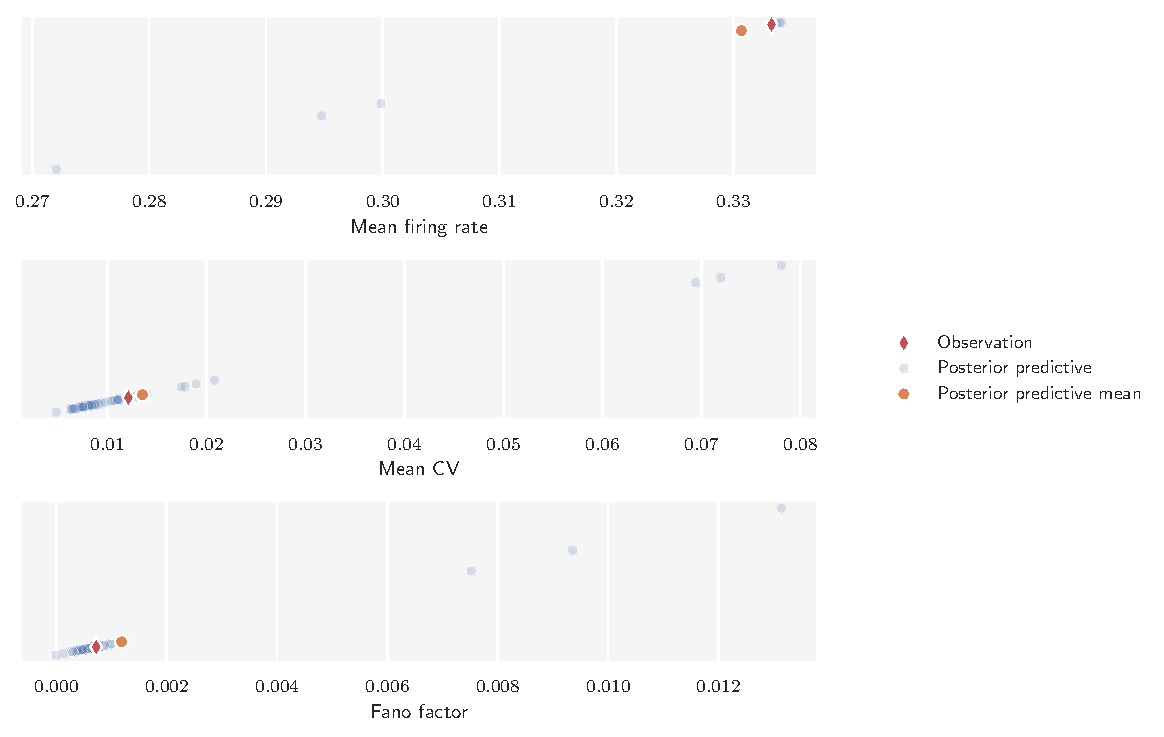
\includegraphics[scale=0.8]{brunel_post_pred_sr_sbi}
    \caption{caption}
    \label{fig:fig1}
\end{figure}

corr 

\begin{figure}[H]
    \centering
    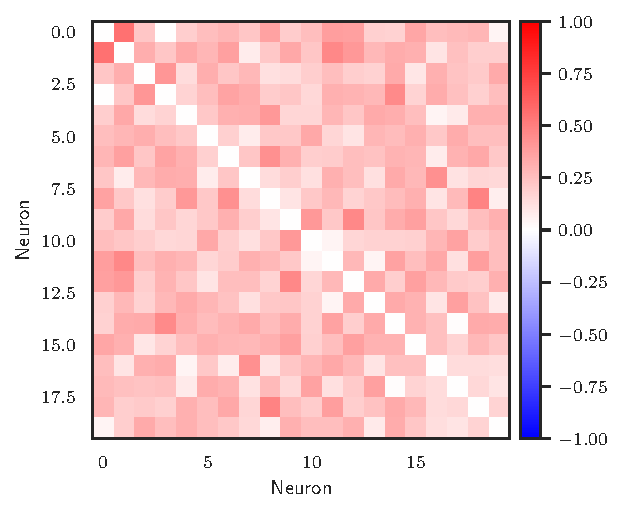
\includegraphics[scale=0.8]{brunel_pred_corr_sbi_sr}
    \caption{caption}
    \label{fig:fig1}
\end{figure}

corr std

\begin{figure}[H]
    \centering
    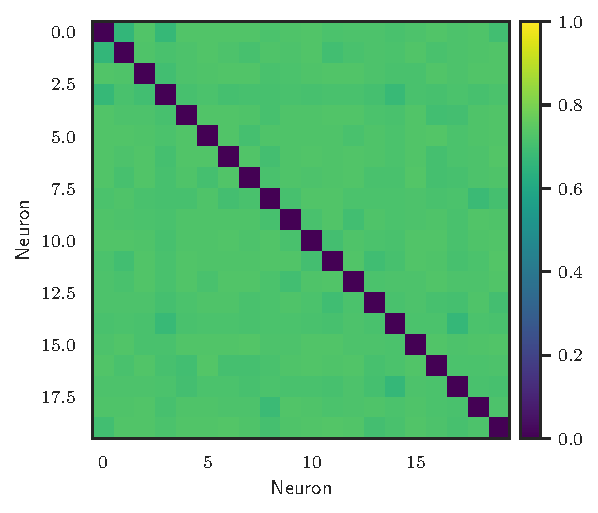
\includegraphics[scale=0.8]{brunel_pred_corr_std_sr_sbi}
    \caption{caption}
    \label{fig:fig1}
\end{figure}
